%% bare_conf.tex
%% V1.3
%% 2007/01/11
%% by Michael Shell
%% See:
%% http://www.michaelshell.org/
%% for current contact information.
%%
%% This is a skeleton file demonstrating the use of IEEEtran.cls
%% (requires IEEEtran.cls version 1.7 or later) with an IEEE conference paper.
%%
%% Support sites:
%% http://www.michaelshell.org/tex/ieeetran/
%% http://www.ctan.org/tex-archive/macros/latex/contrib/IEEEtran/
%% and
%% http://www.ieee.org/

%%*************************************************************************
%% Legal Notice:
%% This code is offered as-is without any warranty either expressed or
%% implied; without even the implied warranty of MERCHANTABILITY or
%% FITNESS FOR A PARTICULAR PURPOSE! 
%% User assumes all risk.
%% In no event shall IEEE or any contributor to this code be liable for
%% any damages or losses, including, but not limited to, incidental,
%% consequential, or any other damages, resulting from the use or misuse
%% of any information contained here.
%%
%% All comments are the opinions of their respective authors and are not
%% necessarily endorsed by the IEEE.
%%
%% This work is distributed under the LaTeX Project Public License (LPPL)
%% ( http://www.latex-project.org/ ) version 1.3, and may be freely used,
%% distributed and modified. A copy of the LPPL, version 1.3, is included
%% in the base LaTeX documentation of all distributions of LaTeX released
%% 2003/12/01 or later.
%% Retain all contribution notices and credits.
%% ** Modified files should be clearly indicated as such, including  **
%% ** renaming them and changing author support contact information. **
%%
%% File list of work: IEEEtran.cls, IEEEtran_HOWTO.pdf, bare_adv.tex,
%%                    bare_conf.tex, bare_jrnl.tex, bare_jrnl_compsoc.tex
%%*************************************************************************

% *** Authors should verify (and, if needed, correct) their LaTeX system  ***
% *** with the testflow diagnostic prior to trusting their LaTeX platform ***
% *** with production work. IEEE's font choices can trigger bugs that do  ***
% *** not appear when using other class files.                            ***
% The testflow support page is at:
% http://www.michaelshell.org/tex/testflow/



\documentclass[conference]{IEEEtran}
% Add the compsoc option for Computer Society conferences.
%
% If IEEEtran.cls has not been installed into the LaTeX system files,
% manually specify the path to it like:
% \documentclass[conference]{../sty/IEEEtran}


% Some very useful LaTeX packages include:
% (uncomment the ones you want to load)

% *** GRAPHICS RELATED PACKAGES ***
%
\usepackage[pdftex]{graphicx}

% *** MATH PACKAGES ***
%
\usepackage[cmex10]{amsmath}

% *** SUBFIGURE PACKAGES ***
%\usepackage[tight,footnotesize]{subfigure}
% subfigure.sty was written by Steven Douglas Cochran. This package makes it
% easy to put subfigures in your figures. e.g., "Figure 1a and 1b". For IEEE
% work, it is a good idea to load it with the tight package option to reduce
% the amount of white space around the subfigures. subfigure.sty is already
% installed on most LaTeX systems. The latest version and documentation can
% be obtained at:
% http://www.ctan.org/tex-archive/obsolete/macros/latex/contrib/subfigure/
% subfigure.sty has been superceeded by subfig.sty.



%\usepackage[caption=false]{caption}
\usepackage[font=footnotesize,caption=false]{subfig}
% subfig.sty, also written by Steven Douglas Cochran, is the modern
% replacement for subfigure.sty. However, subfig.sty requires and
% automatically loads Axel Sommerfeldt's caption.sty which will override
% IEEEtran.cls handling of captions and this will result in nonIEEE style
% figure/table captions. To prevent this problem, be sure and preload
% caption.sty with its "caption=false" package option. This is will preserve
% IEEEtran.cls handing of captions. Version 1.3 (2005/06/28) and later 
% (recommended due to many improvements over 1.2) of subfig.sty supports
% the caption=false option directly:
%\usepackage[caption=false,font=footnotesize]{subfig}
%
% The latest version and documentation can be obtained at:
% http://www.ctan.org/tex-archive/macros/latex/contrib/subfig/
% The latest version and documentation of caption.sty can be obtained at:
% http://www.ctan.org/tex-archive/macros/latex/contrib/caption/


% --------------- USEPACKAGE agregados por guanucoluis ----------------

\usepackage[utf8]{inputenc}
\usepackage{multirow}
%\usepackage[english]{babel}
\usepackage{amssymb}
%\usepackage[pdftex]{graphicx}
\usepackage[hyphenbreaks]{breakurl}
\usepackage[hyphens]{url}
\usepackage{lipsum}
\usepackage{listings}
\lstset{% general command to set parameter(s)
basicstyle=\scriptsize\ttfamily}

\usepackage{textcomp}

% ------------------------- Agregados por maxi ------------------------

\renewcommand{\abstractname}{Resumen}
\renewcommand{\IEEEkeywordsname}{Palabras claves}
\renewcommand{\figurename}{Fig.}
\renewcommand{\tablename}{Tabla}
\renewcommand{\refname}{Referencias}
\hyphenation{de-sa-rro-llar de-sa-rro-llos}

%lista de posibles "Fixed names"  de latex que pueden hacer falta
%\abstractname	 Abstract
%\alsoname	 see also (makeidx package)
%\appendixname	 Appendix
%\bibname	 Bibliography (report,book)
%\ccname	 cc (letter)
%\chaptername	 Chapter (report,book)
%\contentsname	 Contents
%\enclname	 encl (letter)
%\figurename	 Figure (for captions)
%\headtoname	 To (letter)
%\indexname	 Index
%\listfigurename	 List of Figures
%\listtablename	 List of Tables
%\pagename	 Page (letter)
%\partname	 Partnnn
%\refname	 References (article)
%\seename	 see (makeidx package)
%\tablename	 Table (for caption)



% correct bad hyphenation here
\hyphenation{op-tical net-works semi-conduc-tor}

\begin{document}
%
% paper title
% can use linebreaks \\ within to get better formatting as desired
\title{Servicios Web}

% author names and affiliations
% use a multiple column layout for up to three different
% affiliations
\author{\IEEEauthorblockN{Franco Bocalon, Luis Guanuco, Santiago
    Nolasco}
  \IEEEauthorblockA{Sistemas Distribuidos\\
    Especialidad en Sistemas Embebidos\\
    Instituto Universitario Aeronáutico}
}

% use for special paper notices
%\IEEEspecialpapernotice{(Invited Paper)}


% make the title area
\maketitle


\begin{abstract}
  Las arquitecturas de los servicios web fueron evolucionando en
  función de las necesidades tanto de los proveedores como los
  usuarios. La expansión de internet y nuevas tecnologías
  (dispositivos móviles, IoT, etc.) modelaron los sistemas
  actuales. En base a la definición de SOA (Services Object
  Architecture), se enfocará en la importancia y madurez de los
  servicios SOAP (Simple Object Access Protocol) para luego 



Aquí se expone un resumido análisis del \emph{Estado del
    Arte} de los servicios web con el foco en los \emph{Servicios
    REST}.

\end{abstract}

% Note that keywords are not normally used for peerreview papers.
\begin{IEEEkeywords}
Web services, SOA, SOAP, REST.
\end{IEEEkeywords}

% IEEEtran.cls defaults to using nonbold math in the Abstract.
% This preserves the distinction between vectors and scalars. However,
% if the conference you are submitting to favors bold math in the abstract,
% then you can use LaTeX's standard command \boldmath at the very start
% of the abstract to achieve this. Many IEEE journals/conferences frown on
% math in the abstract anyway.

% no keywords

% For peer review papers, you can put extra information on the cover
% page as needed:
% \ifCLASSOPTIONpeerreview
% \begin{center} \bfseries EDICS Category: 3-BBND \end{center}
% \fi
%
% For peerreview papers, this IEEEtran command inserts a page break and
% creates the second title. It will be ignored for other modes.
\IEEEpeerreviewmaketitle

\section{Introducción}

% Conceptos de SOA. Un diagrama ejemplo con servicios web varios.
% Características de SOAP y REST.

En la actualidad, debido a los competitivos mercados globales, las
compañías se ven presionadas a responder de la manera más efectiva
posible. Saber actuar ante los cambios que afectan de manera natural a
los negocios, optimizar los procesos, reducir los costos de IT, y
lograr flexibilidad, son algunos de los factores claves para la
competitividad y el crecimiento de las organizaciones.
Para lograrlo se necesita una herramienta basada en estándares para
integrar sistemas y aplicaciones heterogéneos sobre una serie de
plataformas y protocolos de comunicación, con una metodología bien
establecida. Este marco de trabajo conceptual es SOA
(\textsl{Service-Oriented Architecture}).

\subsection{SOA}
\label{sec:intro-soa}

La Arquitectura Orientada a Servicios supone una estrategia general de
organización de los
elementos de IT, de forma que una colección desordenada de sistemas
distribuidos y aplicaciones complejas se pueda transformar en una red
de recursos integrados, simplificados y sumamente
flexible\cite{SOA1}. Un
proyecto SOA bien ejecutado permite alinear los recursos de IT de
forma más directa con los objetivos de negocio, ganando así un mayor
grado de integración con clientes y proveedores, esto es
descomponiendo toda su estructura en servicios. Los cuales pueden ser
añadidos y también sustraídos sin alterar el complejo sistema. Esta
independencia abstrae al programador de las conexiones entre
plataformas, lenguajes de programación y dependencia de otros
servicios.

Los resultados son la reducción de costos de implementación,
innovación de servicios a clientes, adaptación ágil ante cambios y
reacción temprana ante la competitividad, ya que, combinan fácilmente
las nuevas tecnologías con aplicaciones independientes permitiendo
que los componentes del proceso se integren y coordinen de manera
efectiva y rápida. 

\subsection{SOA vs Arquitectura tradicional}
\label{sec:soa-vs-arq-tra}

En la Tabla \ref{tab:soa-vs-trad} podemos apreciar la diferencia entre
una arquitectura tradicional y el paradigma SOA\cite{SOA2}. La
diferencia sustancial es que en la arquitectura SOA, se busca la
independencia de los servicios. Esta independencia se logra a traves
de la aplicacion de protocolos, logrando un bajo acoplamiento entre
los servicios web.

\begin{table}[!t]
  \renewcommand{\arraystretch}{1.3}
  \caption{Arquitecturas de servicios web.}
  \label{tab:soa-vs-trad}
  \centering
  \begin{tabular}{|l|l|}
    \hline
    \textbf{Arquitectura tradicional} & \textbf{Arquitectura orientada
      a servicios}\\
    \hline\hline
    Forzada a la funcionalidad & Orientado al proceso \\\hline
    Diseñado para durar & Diseñado para el cambio\\\hline
    Desarrollo con largos ciclos de tiempo & Desarrollo
    iterativo\\\hline
    Fuerte acoplamiento & Bajo acoplamiento \\\hline
    Aplicación especifica & Heterogéneo\\\hline
    Orientado a datos & Orientado al servicio empresarial\\
    \hline
  \end{tabular}
\end{table}


% \section{SOAP}
% \label{sec:soap}

\section{Servicios basados en SOA}
\label{sec:serv-soa-based}

El uso más común que se suele dar a este servicio es el de integrar
diferentes sistemas o componentes de una o varias
plataformas. Mediante el uso de estándares se consigue dicha
integración y a la vez  interoperante. La clave se encuentra en el
intercambio de mensajes entre sistemas (Figura
\ref{fig:soa})\cite{SOA3}.


\begin{figure}[!t]
\centering
  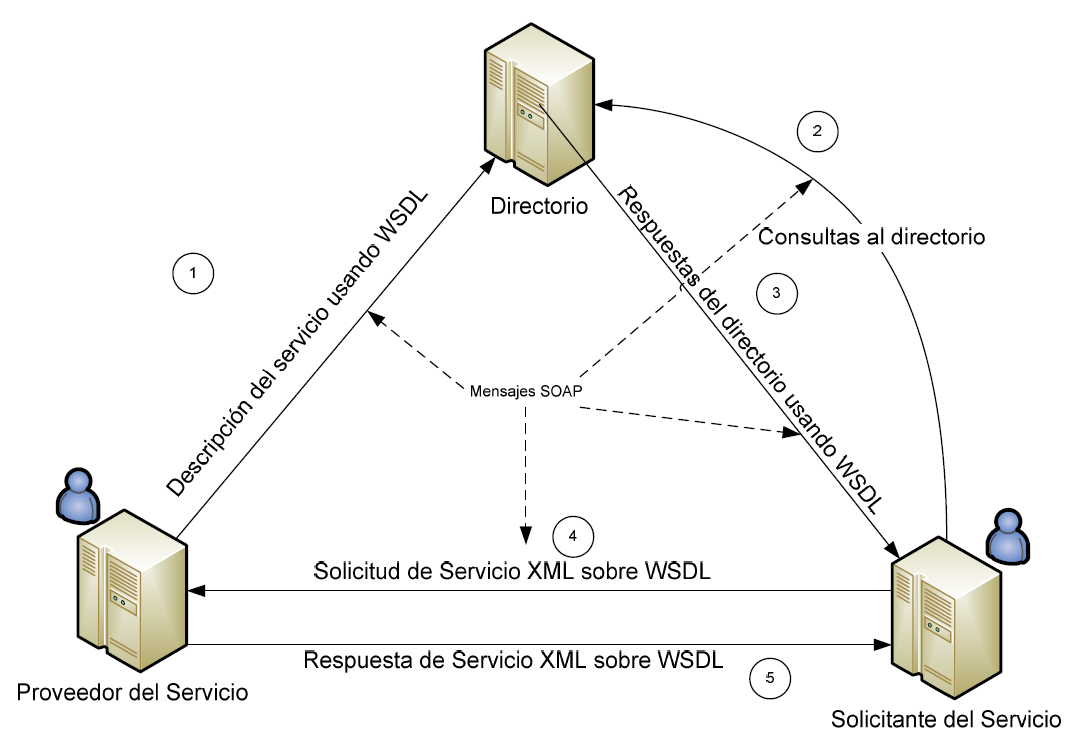
\includegraphics[width=0.5\textwidth]{img/soa}
  \caption{Interacción de mensajes en las arquitecturas SOA.}
  \label{fig:soa}
\end{figure}

Los servicios web se basan en un conjunto de estándares de
comunicación. A continuación se describirán algunos de estos
estándares. 

\subsection{XML}
\label{sec:serv-soa-xml}

Proviene del lenguaje SGML y permite definir la gramática de lenguajes
específicos\footnote{De la misma manera que HTML es a su vez un lenguaje
definido por SGML.} para estructurar documentos grandes. A diferencia
de otros lenguajes, XML da soporte a bases de datos, siendo útil
cuando varias aplicaciones deben comunicarse entre sí o integrar
información.

\subsection{WSDL}
\label{sec:serv-soa-wsdl}

Describe la interfaz pública a los servicios web. Está basado en XML y
describe la forma de comunicación. Es decir, los requisitos del
protocolo y los formatos de los mensajes necesarios para interactuar
con los servicios listados en su catálogo. Las operaciones y mensajes
que soporta se describen en abstracto y se ligan después al protocolo
concreto de red y al formato del mensaje.

WSDL se usa a menudo en combinación con SOAP y XML Schema[REF]. Un programa
cliente que se conecta a un servicio web puede leer el WSDL para
determinar qué funciones están disponibles en el servidor. Los tipos
de datos especiales se incluyen en el archivo WSDL en forma de XML
Schema. El cliente puede usar SOAP para hacer la llamada a una de las
funciones listadas en el WSDL.

\subsection{SOAP}
\label{sec:serv-soa-soap}

SOAP (\textsl{Simple Object Access Protocol}) es usado para el
intercambio de datos.
Es un paradigma de mensajería de una dirección sin estado que puede
ser utilizado para formar protocolos más complejos y completos según
las necesidades de las aplicaciones que lo implementan. Puede formar y
construir la capa base de una \emph{pila de protocolos de web service},
ofreciendo un framework de mensajería básica en el cual los \emph{web
services} pueden ser construidos.

Este protocolo está basado en XML y la estructura consta de tres
partes[REF]:
\begin{itemize}
\item\emph{Envelope}: Qué hay en el mensaje y cómo procesarlo.
\item\emph{Header}: Es una extensión que permite enviar información
  relativa a cómo debe ser procesado el mensaje.
\item\emph{Body}: Contiene la información relativa a la llamada y la
  respuesta.
\end{itemize}

\begin{figure}[!t]
\centering
  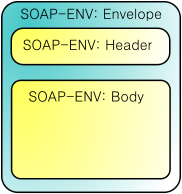
\includegraphics[width=0.15\textwidth]{img/soap}
  \caption{Estructura del mensaje utilizado por SOAP.}
  \label{fig:soap-env}
\end{figure}

El protocolo SOAP tiene tres características principales:
\begin{itemize}
\item\emph{Extensibilidad}: seguridad y WS-routing son extensiones aplicadas
  en el desarrollo.
\item\emph{Neutralidad}: SOAP puede ser utilizado sobre cualquier protocolo
  de transporte como HTTP, SMTP, TCP o JMS.
\item\emph{Independencia}: SOAP permite cualquier modelo de programación.
\end{itemize}

El enfoque del SOAP\cite{SOA4} es encapsular la lógica como solicitud
de la base
de datos para el servicio. A traves de un método (o función) en
cualquier lenguaje como C, VB, Java, etc.; y a continuación establecer
un proceso que escucha las
solicitudes al servicio siendo dichas solicitudes en formato SOAP y
que contienen el nombre del servicio y los parámetros requeridos. La
capa de transporte puede ser HTTP, aunque podría ser fácilmente SMTP o
alguna otra. Entonces, el proceso de escucha, que por simplicidad se
suelen escrito en el mismo lenguaje que el método de servicio,
decodifica la petición SOAP de entrada y la transforma en una
invocación del método.
Luego toma el resultado de la llamada al método, lo codifica en un
mensaje SOAP (respuesta) y lo envía de vuelta al
solicitante. Conceptualmente, esta disposición tiene el aspecto de la
Figura \ref{fig:soap-comp}.

\begin{figure*}[!t]
\centering
  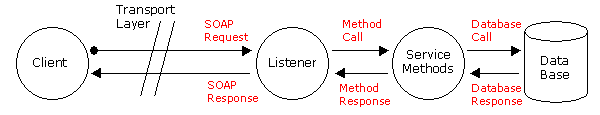
\includegraphics[width=0.8\textwidth]{img/soap-comp}
  \caption{Componentes en un pedido de servicios SOAP.}
  \label{fig:soap-comp}
\end{figure*}

Existen más especificaciones, a las que se denomina genéricamente como
la arquitectura WS-*, que definen distintas funcionalidades para el
descubrimiento de servicios Web, gestión de eventos, archivos
adjuntos, seguridad, gestión y fiabilidad en el intercambio de
mensajes y transacciones. 

\section{REST}
\label{sec:soap}

%Hablamos del paradigma. Implementación. Un ejemplo
REST o \textsl{Representational State Teansfer} fue creado por Roy
Fielding\footnote{\texttt{http://www.ics.uci.edu/\texttildelow fielding/}} en el
año 2000. Este concepto fue expuesto por primera vez en la disertación
de la tesis doctoral de Fielding. En dicha exposición se exploraba
varios estilos arquitectónicos basados en redes. En el Capítulo 5
\cite{FieldingPhD} de sus tesis se hace una descripción profunda. REST
puede ser descrito como una forma de construir servicios Web siguiendo
alguna restricciones entre el proveedor y el cliente de tales
servicios como son\cite{NordicAPIs}:

\begin{itemize}
\item \emph{Mantener separados los intereses entre el cliente y
    servidor}:
  con esto, los clientes no deberían preocuparse por el almacenamiento
  de datos, al igual que los servidores no deben preocuparse por las
  interfaces de usuario. Esto desacopla por completo el desarrollo de
  ambas partes del sistema y permite economizar los recursos en el
  escalamiento. 
\item \emph{La comunicación entre cliente y servidor debería ser ``sin
  estados'' (stateless)}:  los servidores no deberían almacenar
  ninguna información sobre el contexto del cliente en sus
  llamadas. Obviamente con las excepciones de sesiones que utilizan
  información para mantener la autenticación de la conexión.
\item \emph{Los clientes debe almacenar en cache  las respuestas}:
  todas las
  respuestas del servidor deben conener la suficiente información
  relacionada a cache. Por lo tanto, los clientes puede confiar en esa
  información y decidir por sí mismos qué almacenar de la respuesta en
  cache. 
\item \emph{La conexiones pueden producirse  a través de varias capas de
  comunicación}: los clientes no deben ser capaces de distinguir sí
  están directamente conectados al servidor de la aplicación o a un
  agente intermediario que transmite la información. 
\end{itemize}

% \subsection{Simplicidad}
% \label{sec:rest-simp}

La simplicidad de REST puede verse en el siguiente ejemplo. Se pide
obtener los datos de un usuario a partir de su identificador.
Usando la arquitectura SOAP, la petición debería tener la siguiente
forma:
\begin{lstlisting}[frame=single]
<?xml version="1.0"?>
<soap:Envelope
xmlns:soap="http://www.w3.org/2001/12/soap-envelope"
soap:encodingStyle="http://www.w3.org/2001/12/soap-encoding">
 <soap:body pb="http://www.acme.com/phonebook">
  <pb:GetUserDetails>
   <pb:UserID>12345</pb:UserID>
  </pb:GetUserDetails>
 </soap:Body>
</soap:Envelope>
\end{lstlisting}

Esto se envía al servidor utilizando el comando \texttt{HTTP POST}. El
resultado probablemente será un archivo XML, pero esto
se encuentra embebido como la carga-paga, dentro de una respuesta
SOAP.

Y con REST la consulta probablemente sea como la que sigue,
\begin{lstlisting}[frame=single]
http://www.acme.com/phonebook/UserDetails/12345
\end{lstlisting}

En este caso solo se tiene un URL. Este URL se envía al servidor
usando simplemente un pedido de \texttt{GET} y la respuesta en HTTP se
obtiene en bruto. No se adquiere nada más de lo que se pide al
servidor. 

Note como el método del URL no se llama \texttt{GetUserDetails}, es
simplemente \texttt{UserDetails}. Esto es una de las convenciones en
el diseño REST donde se usa  \emph{sustantivos} en vez de
\emph{verbos} para denotar un simple \emph{recurso}.

Una analogía que resume las diferencias entre SOAP y REST es
considerar ambos servicios como el redactar una carta. Donde el uso de
SOAP sería como utilizar \emph{un sobre para enviar la carta}. En
cambio REST podría considerarse una \emph{postal}. Una postal es fácil
de enviar y leerla, además de consumir menos papel.

Con respecto a la seguridad se podría decir que REST es un poco más
seguro que SOAP. En particular, REST podría ser implementado sobre un
socket seguro como ser HTTPS y el contenido podría también estar
encriptado usando cualquier mecanismo existente. De todas formas, sin
encriptación, tanto REST como SOAP son inseguros. 

\section{Comparación de servicios web}
\label{sec:comparacion}

Aquí vamos a poner las ventajas y desventajas entre los servicios REST
y los web services tradicionales.

% \subsection{Casos de uso dónde REST es mejor que SOAP}
% \label{sec:cu-rest-better-soap}

SOAP proporciona formas de acceder y manipular objetos remotos, mientras que REST se focaliza en la operaciones que puede ser
ejecutada sobre los recursos. Esta característica hace que REST tenga
mayor adopción en APIs. Además, porque REST hereda operaciones del
protocolo HTTP. Esto último hace fácil la elección de ``cómo abrir una
API web''. Estas características han influido tanto que grandes
compañías Web utilizan la API REST\footnote{RESTful es el nombre
  técnico de la implementación de REST.}.

REST es mejor que SOAP en situaciones que no requieren un mapeo total
de los objetos al cliente. La comunicación de información de objetos
en ambos sentidos demanda una cantidad importante de ancho de banda,
lo que podría ser una limitante en entornos donde la conectividad es
costosa. Una API requerida principalmente para aplicaciones móviles es
uno de los casos de uso donde se debe evitar el uso de SOAP.

Otro factor en la preferencia a REST es la simplicidad de la
implementación con respecto a SOAP. También, al ser menos restrictivo
que SOAP, algunas APIs de REST trabajan mejor en la actualidad. En
algunos casos los desarrolladores no conocen en profundidad los
contratos a la hora de implementar una API. Las APIs públicas cambian
constantemente debido a las necesidades de negocio y son adaptables
rápidamente. En esta situación REST resulta una elección
natural. El uso de SOAP en las condiciones expuestas sería
contraproducente ya que podría introducir una complejidad contractual
innecesaria. 

Actualmente es común leer el término \emph{ROA} (REST Oriented
Architecture). ROA es simplemente el nombre que se le da a los
servicios SOA (Service Based Architecture) que utilizan REST.

La principal ventaja de SOA sobre ROA es la madurez de las
herramientas. Sin embargo, esto ha cambiado con el tiempo. En la
actualidad la mayoría de los servicios web se basan en REST.

Como se dijo anteriormente, la principal ventaja de REST es la
facilidad en su implementación, agilidad en el diseño y el enfoque
sencillo en el manejo de recursos. En cambio, SOAP tiene un perfil
orientado a servicios para empresas. Aquí se pueden encontrar usos en
bancos e industrias financieras. Contrariamente, si alguien necesita
montar rápidamente un servicio con un buen funcionamiento y baja
demanda de recursos, seguramente elegirán REST.

\section{Conclusiones}
\label{sec:con}
\lipsum[1]
\begin{thebibliography}{1}

% \bibitem{IEEEhowto:kopka}
% H.~Kopka and P.~W. Daly, \emph{A Guide to \LaTeX}, 3rd~ed.\hskip 1em plus
%   0.5em minus 0.4em\relax Harlow, England: Addison-Wesley, 1999.

\bibitem{FieldingPhD}
  Roy~Fielding, \emph{Architectural Styles and the Design of
    Network-based Software Architectures}. University of California,
  Irvine. 2000. url:\texttt{\burl{http://www.ics.uci.edu/\texttildelow
      fielding/pubs/dissertation/rest_arch_style.htm}}.

\bibitem{NordicAPIs}
Bruno~Pedro, \emph{Is REST better than SOAP? Yes, in Some Use Cases},
url:
\texttt{\burl{http://nordicapis.com/rest-better-than-soap-yes-use-cases/}}.

\bibitem{LearnREST}
  Dr. M. Elkstein, \emph{Learn REST: A Tutorial},
url: \texttt{\burl{http://rest.elkstein.org/}}.

\bibitem{SOA1}
  Whitepaper, \emph{La Arquitectura SOA de Microsoft Aplicada al Mundo
  Real}.

\bibitem{SOA2}
  Umair~Ashraf, \emph{CS 415 N-Tier Application Development}. National
  University of Computer and Emerging Sciences. July 5, 2013.

\bibitem{SOA3}
  Miguel Rodríguez, \emph{SOA vs SOAP y REST}. url:
  \texttt{\burl{http://www.adictosaltrabajo.com/tutoriales/soavs-soap-rest/}}.

\bibitem{SOA4}
  Nicholas Quaine, \emph{ SOAP Basics -- What is SOAP? }. url:
  \texttt{\burl{http://www.soapuser.com/basics1.html}}.

\end{thebibliography}

% that's all folks
\end{document}


